\section{Proposed}
\label{Pro}

\subsection{Dirty Ancilla Node Gadgets}
\label{sub-synth}
Here we take the dirty ancilla construction in~\ref{sub-mct}, and create a gadget to
realize an XAG AND node using dirty ancilla. First, we separate the construction into
two parts, as in~\figref{fig-dirt-mct-org}: we label these \emph{compute}, and \emph{uncompute}.
We observe that the Toffoli gate in compute can be replaced with a single target controlled
gate for an arbitrary function F; that is, it's a gate that flips its target bit when a
function F is true. We can implement this function F as a quantum
subcircuit~\cite{bib-amy-phase-state}, and so we can realize a recursive construction, depicted
in~\figref{fig-compute}. The Toffoli gate in the uncompute gadget can thus be replaced with the
gate F's adjoint. For a relative phase gate, this means implementing F's components' adjoints in
reverse, to realize a gate that implements the same function, but with the opposite relative phase
~\cite{bib-maslov-rtof}.

\begin{figure}[t]
  \centering
  \scalebox{1.0} {
    \begin{quantikz}[row sep=0.5em, column sep=0.5em]
  \setwiretype{n}    &     &                                                                                                                                                                 & \push{Compute} &          &  & \push{Uncompute}                                                                                                                                                     &  &  \\
  \setwiretype{n}    &     &                                                                                                                                                                 &                &          &  &                                                                                                                                                                      &  &  \\  
  \lstick{\ket{x_0}} & \qw & \qw \gategroup[5,steps=3,style={dashed,rounded corners,fill=blue!20, inner xsep=2pt},background,label style={label position=above,anchor=north,yshift=-0.2cm}]{}& \ctrl{1}       & \qw      &  & \ctrl{1} \gategroup[5,steps=2,style={dashed,rounded corners,fill=red!20, inner xsep=2pt},background,label style={label position=above,anchor=north,yshift=-0.2cm}]{} &  & \rstick{\ket{x_0}} \\
  \lstick{\ket{x_1}} & \qw & \qw                                                                                                                                                             & \ctrl{2}       & \qw      &  & \ctrl{2}                                                                                                                                                             &  & \rstick{\ket{x_1}} \\
  \lstick{\ket{x_2}} & \qw & \ctrl{1}                                                                                                                                                        & \qw            & \ctrl{1} &  & \qw                                                                                                                                                                  &  & \rstick{\ket{x_2}} \\
  \lstick{a}         & \qw & \ctrl{1}                                                                                                                                                        & \targ{}        & \ctrl{1} &  & \targ{}                                                                                                                                                              &  & \rstick{a} \\  
  \lstick{\ket{y}}   & \qw & \targ{}                                                                                                                                                         & \qw            & \targ{}  &  & \qw                                                                                                                                                                  &  & \rstick{\ket{x_0 \cdot x_1 \oplus y}}  
\end{quantikz}

%% \begin{quantikz}[row sep=0.5em, column sep=0.5em]
%%   \lstick{\ket{x_0}} & \qw & \qw      & \ctrl{1} & \qw      & \ctrl{1} & \qw & \rstick{\ket{x_0}} \\
%%   \lstick{\ket{x_1}} & \qw & \qw      & \ctrl{2} & \qw      & \ctrl{2} & \qw & \rstick{\ket{x_1}} \\
%%   \lstick{\ket{x_2}} & \qw & \ctrl{1}\gategroup[5,steps=3,style={dashed,rounded corners},label style={above}]{Compute} & \qw      & \ctrl{1} & \qw      & \qw & \rstick{\ket{x_2}} \\
%%   \lstick{a}         & \qw & \ctrl{1} & \targ{}  & \ctrl{1} & \targ{}  &     & \rstick{a} \\  
%%   \lstick{\ket{y}}   & \qw & \targ{}  & \qw      & \targ{}\gategroup[5,steps=1,style={dashed,rounded corners},label style={above}]{Uncompute} & \qw      & \qw & \rstick{\ket{x_0 \cdot x_1 \oplus y}}  \\
%% \end{quantikz}
%% \begin{quantikz}[row sep=0.5em, column sep=0.5em]
%%   \lstick{\ket{x_0}} & \qw & \qw      & \ctrl{1} & \qw      & \ctrl{1} & \qw & \rstick{\ket{x_0}} \\
%%   \lstick{\ket{x_1}} & \qw & \qw      & \ctrl{2} & \qw      & \ctrl{2} & \qw & \rstick{\ket{x_1}} \\
%%   \lstick{\ket{x_2}} & \qw & \ctrl{1} & \qw      & \ctrl{1} & \qw      & \qw & \rstick{\ket{x_2}} \\
%%   \lstick{a}         & \qw & \ctrl{1} & \targ{}  & \ctrl{1} & \targ{}  &  & \rstick{a} \\  
%%   \lstick{\ket{y}}   & \qw & \targ{}  & \qw      & \targ{}  & \qw      & \qw & \rstick{\ket{x_0 \cdot x_1 \oplus y}}  \\
%% \end{quantikz}                        


  }
  \caption{Dirty MCT decomposition base}
  \label{fig-dirt-mct-org}
\end{figure}

\begin{figure}[t]
  \centering
  \scalebox{1.0} {
    \begin{quantikz}[row sep=0.3cm, column sep=0.3cm]
\qw              & \qw             & \qw        & \gate[2]{F}         & \qw               & \qw      & \qw    \\
\qw              & \qw             & \qw        & \ghost{F}\ctrl{2}   & \qw               & \qw      & \qw    \\
\lstick{$G$}     & \qw             & \ctrl{1}   & \qw                 & \ctrl{1}          & \qw      & \qw    \\
\lstick{$a_0$}   & \qw             & \gate{Z}   & \targ{}             & \gate{Z^\dagger}  & \qw      & \qw    \\
\lstick{$t$}     & \gate{H}        & \ctrl{-1}  & \qw                 & \ctrl{-1}         & \gate{H} & \qw    \\
\end{quantikz}

%% \begin{quantikz}[row sep=0.3cm, column sep=0.55cm]
%% \qw              & \qw             & \qw        & \qw             & \qw              & \gate[2]{F_i}       & \qw                    & \qw       & \qw             & \qw      & \qw        & \qw              & \gate[2]{F_i}        & \qw                     & \qw        \\
%% \qw              & \qw             & \qw        & \qw             & \qw              & \ghost{F_i}         & \qw                    & \qw       & \qw             & \qw      & \qw        & \qw              & \ghost{F_i}          & \qw                     & \qw        \\
%% \qw              & \qw             & \qw        & \qw             & \ctrl{2}         & \qw                 & \ctrl{2}               & \qw       & \qw             & \qw      & \qw        & \ctrl{2}         & \qw                 & \ctrl{2}                & \qw         \\
%% \qw              & \qw             & \octrl{2}  & \qw             & \qw              & \qw                 & \qw                    & \qw       & \qw             & \qw      & \qw        & \qw              & \qw                 & \qw                     & \qw         \\
%% \lstick{$a_1$}   & \qw             & \qw        & \qw             & \gate{i\omega Z} & \targ{}             & \gate{i\omega Z^\dagger} & \qw       & \octrl{1}       & \qw      & \qw        & \gate{i\omega Z} & \targ{}             & \gate{i\omega Z^\dagger}  & \qw          \\
%% \lstick{$a_2$}   & \qw             & \gate{iZ}  & \gate{H}        & \ctrl{-1}        & \qw                 & \ctrl{-1}              & \gate{H}  & \gate{iZ^\dagger} & \qw      & \gate{H}   & \ctrl{-1}        & \qw                 & \ctrl{-1}               & \gate{H}     \\
%% \lstick{}        & \gate{H}        & \ctrl{-1}  & \qw             & \qw              & \qw                 & \qw                    & \qw       & \ctrl{-1}       & \gate{H} & \qw        & \qw              & \qw                 & \qw                     & \qw          \\
%%\end{quantikz}


  }
  \caption{Compute gadget}
  \label{fig-compute}
\end{figure}

We utilize the fact that the CCZ has two complementary implementations to our advantage by replacing the left CCZ
gate with~\figref{fig-cnot-t-ccz} and the right with \figref{fig-alt-cnot-t-ccz}. In so doing we can combine their
sum-of-paths to get the below sum-of-paths equation:

\begin{equation}
  \label{eq-toff-tot}
  \begin{aligned}
    &\frac{1}{4}z + \frac{1}{4}a + \frac{1}{4}f - \frac{1}{4}(z \oplus a) \\
    &\qquad -\frac{1}{4}(z \oplus f) - \frac{1}{4}(a \oplus f) + \frac{1}{4}(z \oplus a \oplus f)\\
    &- \frac{1}{4}z - \frac{1}{4}(xy \oplus a) - \frac{1}{4} f + \frac{1}{4}(z \oplus xy \oplus a) \\
    &\qquad + \frac{1}{4}(z \oplus f) + \frac{1}{4}(xy \oplus a \oplus f) - \frac{1}{4}(z \oplus xy \oplus a \oplus f)
  \end{aligned}
\end{equation}

This causes some cancellations, and we are left with:

\begin{equation}
  \label{eq-toff-simp}
  \begin{aligned}
    &\frac{1}{4}a - \frac{1}{4}(z \oplus a) - \frac{1}{4}(xy \oplus a) + \frac{1}{4}(z \oplus xy \oplus a)  \\
    &+ \frac{1}{4}(z \oplus a \oplus f) - \frac{1}{4}(a \oplus f) + \frac{1}{4}(xy \oplus a \oplus f) \\
    &- \frac{1}{4}(z \oplus xy \oplus a \oplus f)
  \end{aligned}
\end{equation}

Observe that the first line in\eqnref{eq-toff-simp} contains only terms that have no dependence on $f$.
That means we can bring them out from the summation to create a relative phase version of the compute
gadget, which we depict in~\figref{fig-dirty-gadget-rp}. This means that we can implement the compute
gadget with the same T-count as a relative phase Toffoli gate. We can similarly formulate an uncompute
gadget that is this gadget's conjugate, in order to uncompute the value for the same cost. This implies
that any intermediate computation using dirty ancilla can be performed with the same cost as a relative
phase Toffoli gate. 

The output node will have to implement all 8 terms in~\eqnref{eq-toff-simp}. This means that the T-count of
implementing the output node gadget is 8, so that the difference in T-count between the clean ancilla and
the dirty ancilla decompositions is dependent on the number of these output nodes, which is the number of
output bits of the Boolean function $m$. This means that for an MCT gate, the difference between clean
ancilla and dirty ancilla is 1 T-gate. We can implement these as two RTOF gates.

\begin{table*}[t]
\centering
\scalebox{0.9}{
  \begin{tabular}{p{0.05\textwidth}|p{0.10\textwidth}|p{0.10\textwidth}|p{0.75\textwidth}}
    \# & Node & Conditions & Gadget \\\hline
       {1}
       &
       \scalebox{1.0} {
         \input{xag_and}
       }
       &
       One of A or B are primary inputs and the other is a fanin from another node.
       All fanouts F are intermediate fanouts
       &
       \scalebox{0.9} {
         \input{fig-prop-and}
       }\\\hline
       {2}
       &
       \scalebox{1.0} {
         \input{xag_and}
       }
       &
       Both A and B are fanins from other nodes
       &
       \scalebox{0.9} {
         \begin{quantikz}[row sep=0.2em, column sep=0.5em]
\qw                & \gate[2]{B}              & \gate[2]{B}              & \qw             &                    & \setwiretype{n} & \setwiretype{n} & \setwiretype{n} & \setwiretype{q} & \qw           & \gate[2]{B}       & \qw          & \qw           & \qw                & \qw           & \gate[2]{A}            & \qw           & \qw                & \qw           & \qw            & \qw           & \qw                     \\
\qw                & \ghost{B}\ctrl{2}        & \ghost{B}\ctrl{2}        & \qw             &                    & \setwiretype{n} & \setwiretype{n} & \setwiretype{n} & \setwiretype{q} & \qw           & \ghost{B}\ctrl{2} & \qw          & \qw           & \qw                & \qw           & \ghost{A}\ctrl{2}      & \qw           & \qw                & \qw           & \qw            & \qw           & \qw                     \\
\setwiretype{n}    & \setwiretype{n}          & \setwiretype{n}          & \setwiretype{n} &                    & \push{=}        &                 &                 & \setwiretype{n} & \push{\vdots} & \setwiretype{n}   & \push{\vdots}& \push{\vdots} & \push{\vdots}      & \push{\vdots} & \push{\vdots}          & \push{\vdots} & \push{\vdots}      & \push{\vdots} & \push{\vdots}  & \push{\vdots} & \push{\vdots}               \\
\lstick{$\ket{0}$} & \targ{}                  & \gate[1]{\wedge}\ctrl{2} & \qw             & \push{B}           & \setwiretype{n} & \setwiretype{n} & \setwiretype{n} & \setwiretype{q} & \qw           & \targ{}           & \qw          & \targ{}       & \gate{T}           & \ctrl{1}      & \targ[style={double}]{}& \ctrl{1}      & \gate{T^{\dagger}} & \targ{ }      & \qw            & \qw           & \qw   \\
\lstick{$a$}       &                          & \targX{}                 & \qw             & \push{A \oplus a}  & \setwiretype{n} & \setwiretype{n} & \setwiretype{n} & \setwiretype{q} & \qw           &                   & \targ{}      & \ctrl{-1}     & \gate{T^{\dagger}} & \targ{}       & \qw                    & \targ{}       & \gate{T}           & \ctrl{-1}     & \targ{}        & \qw           & \qw   \\
\lstick{$f$}       &                          & \targ[style={double}]{}  & \qw             & \push{AB \oplus f} & \setwiretype{n} & \setwiretype{n} & \setwiretype{n} & \setwiretype{q} & \gate{H}      &                   & \ctrl{-1}    & \qw           & \qw                & \qw           & \qw                    & \qw           & \qw                & \qw           & \ctrl{-1}      & \gate{H}      & \qw         
\end{quantikz}

%% \begin{quantikz}[row sep=0.3cm, column sep=0.55cm]
%% \qw              & \qw             & \qw        & \qw             & \qw              & \gate[2]{F_i}       & \qw                    & \qw       & \qw             & \qw      & \qw        & \qw              & \gate[2]{F_i}        & \qw                     & \qw        \\
%% \qw              & \qw             & \qw        & \qw             & \qw              & \ghost{F_i}         & \qw                    & \qw       & \qw             & \qw      & \qw        & \qw              & \ghost{F_i}          & \qw                     & \qw        \\
%% \qw              & \qw             & \qw        & \qw             & \ctrl{2}         & \qw                 & \ctrl{2}               & \qw       & \qw             & \qw      & \qw        & \ctrl{2}         & \qw                 & \ctrl{2}                & \qw         \\
%% \qw              & \qw             & \octrl{2}  & \qw             & \qw              & \qw                 & \qw                    & \qw       & \qw             & \qw      & \qw        & \qw              & \qw                 & \qw                     & \qw         \\
%% \lstick{$a_1$}   & \qw             & \qw        & \qw             & \gate{i\omega Z} & \targ{}             & \gate{i\omega Z^\dagger} & \qw       & \octrl{1}       & \qw      & \qw        & \gate{i\omega Z} & \targ{}             & \gate{i\omega Z^\dagger}  & \qw          \\
%% \lstick{$a_2$}   & \qw             & \gate{iZ}  & \gate{H}        & \ctrl{-1}        & \qw                 & \ctrl{-1}              & \gate{H}  & \gate{iZ^\dagger} & \qw      & \gate{H}   & \ctrl{-1}        & \qw                 & \ctrl{-1}               & \gate{H}     \\
%% \lstick{}        & \gate{H}        & \ctrl{-1}  & \qw             & \qw              & \qw                 & \qw                    & \qw       & \ctrl{-1}       & \gate{H} & \qw        & \qw              & \qw                 & \qw                     & \qw          \\
%%\end{quantikz}


       }\\\hline
       {3}
       &
       \scalebox{1.0} {
         \input{xag_and}
       }
       &
       A and B are primary inputs
       &
       \scalebox{1.0} {
         %% \begin{quantikz}[row sep=0.25cm, column sep=0.35cm]
%% \lstick{} & \ctrl{2}  & \lstick{} &\ghost{\qw}         & \ghost{\qw} & \qw & \qw                & \targ{}   & \qw      & \ctrl{1} & \gate{T}           & \ctrl{1} & \qw      & \targ{}    & \qw \\
%% \lstick{} & \ctrl{1}  & \lstick{} &\push{=} & \ghost{\qw} & \qw & \qw                & \qw       & \ctrl{1} & \targ{}  & \gate{T^{\dagger}} & \targ{}  & \ctrl{1} & \qw        & \qw \\
%% \lstick{} & \gate{iZ} & \lstick{} &\push{ } & \ghost{\qw} & \qw & \gate{T^{\dagger}} & \ctrl{-2} & \targ{}  & \qw      & \gate{T}           & \qw      & \targ{}  & \ctrl{-2}  & \qw 
%% \end{quantikz}
\begin{quantikz}[row sep=0.25cm, column sep=0.35cm]
\lstick{$\ket{x_a}$} & \ctrl{1}                & \setwiretype{n} &          && \setwiretype{q} & \qw &          & \qw & \qw                & \targ{}   & \qw      & \ctrl{1} & \gate{T}           & \ctrl{1} & \qw      & \targ{}    &          & \qw \\
\lstick{$\ket{x_b}$} & \ctrl{1}                & \setwiretype{n} & \push{=} && \setwiretype{q} & \qw &          & \qw & \qw                & \qw       & \ctrl{1} & \targ{}  & \gate{T^{\dagger}} & \targ{}  & \ctrl{1} & \qw        &          & \qw \\
\lstick{$\ket{x_c}$} & \targ[style={double}]{} & \setwiretype{n} &          && \setwiretype{q} & \qw & \gate{H} & \qw & \gate{T^{\dagger}} & \ctrl{-2} & \targ{}  & \qw      & \gate{T}           & \qw      & \targ{}  & \ctrl{-2}  & \gate{H} & \qw \\
\end{quantikz}


       }\\\hline
       {4}
       &
       \scalebox{1.0} {
         \input{xag_and}
       }
       &
       F is a primary output or fans out into an XOR node that is a primary output
       &
       \scalebox{0.9} {
         \begin{quantikz}[row sep=0.3cm, column sep=0.55cm]
\qw                & \gate[2]{A}              & \qw             &                     & \setwiretype{n} & \setwiretype{n} & \setwiretype{n} & \setwiretype{q} & \qw                    & \gate[3]{A}       & \qw                    & \qw \\
\qw                & \ghost{A}\ctrl{2}        & \qw             &                     & \setwiretype{n} & \setwiretype{n} & \setwiretype{n} & \setwiretype{q} & \qw                    & \ghost{A}\ctrl{3} & \qw                    & \qw \\
\setwiretype{n}    & \setwiretype{n}          & \setwiretype{n} &                     & \push{=}        &                 &                 & \setwiretype{n} &                        &                   &                        &     \\
\lstick{$B$}       & \gate[1]{\wedge}\ctrl{2} & \qw             & \push{B}            & \setwiretype{n} & \setwiretype{n} & \setwiretype{n} & \setwiretype{q} & \ctrl{1}               & \qw               & \ctrl{1}               & \qw \\
\lstick{$a_i$}     & \targX{}                 & \qw             & \push{A \oplus a_i} & \setwiretype{n} & \setwiretype{n} & \setwiretype{n} & \setwiretype{q} & \ctrl{1}               & \targ{}           & \ctrl{1}               & \qw \\
\lstick{$f$}       & \targ{}                  & \qw             & \push{AB \oplus f}  & \setwiretype{n} & \setwiretype{n} & \setwiretype{n} & \setwiretype{q} & \targ[style={double}]{}& \qw               & \targ[style={double}]{}& \qw  \\
\end{quantikz}

%% \begin{quantikz}[row sep=0.3cm, column sep=0.55cm]
%% \qw              & \qw             & \qw        & \qw             & \qw              & \gate[2]{F_i}       & \qw                    & \qw       & \qw             & \qw      & \qw        & \qw              & \gate[2]{F_i}        & \qw                     & \qw        \\
%% \qw              & \qw             & \qw        & \qw             & \qw              & \ghost{F_i}         & \qw                    & \qw       & \qw             & \qw      & \qw        & \qw              & \ghost{F_i}          & \qw                     & \qw        \\
%% \qw              & \qw             & \qw        & \qw             & \ctrl{2}         & \qw                 & \ctrl{2}               & \qw       & \qw             & \qw      & \qw        & \ctrl{2}         & \qw                 & \ctrl{2}                & \qw         \\
%% \qw              & \qw             & \octrl{2}  & \qw             & \qw              & \qw                 & \qw                    & \qw       & \qw             & \qw      & \qw        & \qw              & \qw                 & \qw                     & \qw         \\
%% \lstick{$a_1$}   & \qw             & \qw        & \qw             & \gate{i\omega Z} & \targ{}             & \gate{i\omega Z^\dagger} & \qw       & \octrl{1}       & \qw      & \qw        & \gate{i\omega Z} & \targ{}             & \gate{i\omega Z^\dagger}  & \qw          \\
%% \lstick{$a_2$}   & \qw             & \gate{iZ}  & \gate{H}        & \ctrl{-1}        & \qw                 & \ctrl{-1}              & \gate{H}  & \gate{iZ^\dagger} & \qw      & \gate{H}   & \ctrl{-1}        & \qw                 & \ctrl{-1}               & \gate{H}     \\
%% \lstick{}        & \gate{H}        & \ctrl{-1}  & \qw             & \qw              & \qw                 & \qw                    & \qw       & \ctrl{-1}       & \gate{H} & \qw        & \qw              & \qw                 & \qw                     & \qw          \\
%%\end{quantikz}


       }\\\hline
       {4}
       &
       \scalebox{1.0} {
         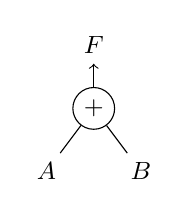
\begin{tikzpicture}[
    gate/.style={circle, draw, inner sep=2pt},
    every node/.style={font=\small}
]

% Inputs
\node (x1) at (0,0) {$A$};
\node (x2) at (1.2,0) {$B$};
\node (x3) at (0.6,1.6) {$F$};

% XOR(x1,x2)
\node[gate] (xor12) at (0.6,0.8) {$+$};
\draw (x1) -- (xor12);
\draw (x2) -- (xor12);
\draw[->] (xor12) -- (x3);

\end{tikzpicture}

       }
       &
       Any XOR node
       &
       \scalebox{1.0} {
         \begin{quantikz}[row sep=0.3cm, column sep=0.55cm]
\qw            & \qw                  & \qw                & \qw   \\
\qw            & \gate[3]{B}          & \gate[3]{A}        & \qw  \\
\qw            & \ghost{B}            & \ghost{A}          & \qw \\
\qw            & \ghost{B}\ctrl{1}    & \ghost{A}\ctrl{1}  & \qw    \\
\qw            & \targ{}              & \targ{}            & \qw  \\
\end{quantikz}
%% \begin{quantikz}[row sep=0.3cm, column sep=0.55cm]
%% \qw            & \qw                            & \gate[3]{A}          & \qw                            & \gate[3]{A}       & \qw   \\
%% \qw            & \gate[3]{B\cdot a_0}         & \ghost{A}            & \gate[3]{B\cdot a_0}         & \ghost{A}         & \qw  \\
%% \qw            & \ghost{B\cdot a_0}           & \ghost{A}\ctrl{1}    & \ghost{B\cdot a_0}           & \ghost{A}\ctrl{1} & \qw \\
%% \lstick{$a_0$} & \ghost{B\cdot a_0}\ctrl{1}   & \targ{}                & \ghost{B\cdot a_0}\ctrl{1}   & \targ{}             & \qw    \\
%% \qw            & \targ{}                        & \qw                    & \targ{}                        & \qw                 & \qw  \\
%% \end{quantikz}


       }
  \end{tabular}
}
\caption{Dirty Ancilla Gadgets}
\label{fig-gadgets}
\end{table*}

%% \begin{table*}[t]
%% \centering
%% \begin{tabular}{p{0.25\textwidth}|p{0.24\textwidth}|p{1.5\textwidth}}
%%   Node & Conditions & Gadget \\\hline
%%   \subfloat[AND-node]{
%%     \makebox[0.25\textwidth][c]{\input{xag_and_node}
%%   }
%%   &
%%   F and G are primary inputs and all fanouts are intermediate fanouts
%%   &
%%   \subfloat[AND-gadget]{
%%     \makebox[\textwidth][c]{\input{fig-prop-and}}
%%   }
%% \end{tabular}
%% \caption{Phase Gadgets}
%% \label{fig-gadgets}
%% \end{table*}


%% The output node will have to implement all 8 terms in~\eqnref{eq-toff-simp}. Observe, however that
%% $\frac{1}{4}a - \frac{1}{4}(z \oplus a) = - \frac{1}{4}z + \frac{1}{2}(a)$. The $\frac{1}{2}$ coefficient
%% can be implemented by an S gate, which is a Clifford gate and has a much more efficient fault-tolerant
%% implementation in most error correcting codes. This means that the T-count of implementing the output
%% node gadget is 7, the exact same as the Toffoli gate which is used as an output node in clean ancilla
%% decomposition.

\begin{figure}
  \scalebox{0.6} {
    \input{fig-prop-and}
  }
  \caption{Relative Phase version of dirty ancilla intermediate compute gadget}
  \label{fig-dirty-gadget-rp}
\end{figure}

\subsection{Proposed Method}

Our proposed method is as follows

\begin{enumerate}
\item Get the next node in the traversal of the XAG, usually from the input
\item Create a subcircuit according to~\tabref{fig-gadgets}
\item Pass on this subcircuit to the next iteration of the algorithm
\item If this node fans out into a primary output, or an XOR node that fans out
  into a primary output take the complement of the passed down subcircuit and set
  it to act on the ancilla that the node uses.
\item If the node is dependent on another subcircuit/subgraph, block until that subcircuit is
  processed.
\item Terminate when all nodes have been processed.
\end{enumerate}

\begin{example}
  \label{ex-dirty-xag}
  We again generate the XAG for~\figref{fig-xag}. Starting from $x_5$ and $x_4$, we
  generate the node they feed into as an RTOF, and pass this RTOF onto the next stage of the iteration.
  We also generate the node taking in $x_2$ and $x_3$, and see that it feeds into an XOR node that
  fans out into a primary output. We generate a Toffoli, and block for the other input.
  We next generate that node's fanout to $x_3$, Because this takes in a fanin from a primary
  input and another node, we plug the RTOF passed down from the previous iteration as $A$
  in gadget\#1, and pass this subcircuit down to the next part of the iteration. We move onto
  the XOR node taking in $x_2$. Since that is an XOR, we generate a subcircuit using a CNOT with
  $x_2$ as an input and replace it in gadget\#4 along with the passed down subcircuit, and pass this
  subcircuit down further. We again repeat the AND procedure for the $x_1$ node the XOR feeds into,
  and feed that output to the next step. Once we have reached the last XOR node, we process both
  the Toffoli feeding into it and the other branch, and generate the full circuit. The full circuit
  is depicted in~\figref{fig-prop-decomp}. We can verify from this diagram that the T-count of this
  is indeed 1 more than the T-count of~\figref{fig-xag-qc} after optimizing it to use RTOF to reduce
  its T-count.
\end{example}

\begin{figure*}[t]
  \centering
  \scalebox{0.8} {
    \begin{quantikz}[row sep=0.2cm, column sep=0.2cm]
\lstick{$x_5$}     & \qw                     & \qw      & \qw             & \qw      &           &                    & \ctrl{1}               &                    &           & \qw       & \qw                      & \qw       & \qw                     & \qw       & \qw             & \qw      &           &                    & \ctrl{1}               &                    &           & \qw       & \qw      & \qw       \\
\lstick{$x_4$}     & \qw                     & \qw      & \qw             & \qw      &           &                    & \ctrl{1}               &                    &           & \qw       & \qw                      & \qw       & \qw                     & \qw       & \qw             & \qw      &           &                    & \ctrl{2}               &                    &           & \qw       & \qw      & \qw       \\
\lstick{$x_3$}     & \qw                     & \qw      & \qw             & \qw      & \targ{}   & \gate{T}           & \targ[style={double}]{}& \gate{T^{\dagger}} & \targ{}   & \qw       & \ctrl{2}                 & \qw       & \qw                     & \ctrl{5}  & \qw             & \qw      & \targ{}   & \gate{T^{\dagger}} & \targ[style={double}]{}& \gate{T}           & \targ{}   & \qw       & \qw      & \qw   \\
\lstick{$x_2$}     & \qw                     & \ctrl{3} & \qw             & \qw      &           &                    & \qw                    &                    &           & \qw       & \qw                      & \qw       & \qw                     & \ctrl{4}  & \qw             & \qw      &           &                    & \qw                    &                    &           & \qw       & \qw      & \ctrl{3}       \\
\lstick{$x_1$}     & \ctrl{1}                &          & \qw             & \qw      &           &                    & \qw                    &                    &           & \qw       & \qw                      & \qw       & \ctrl{1}                & \qw       & \qw             & \qw      &           &                    & \qw                    &                    &           & \qw       & \qw      & \qw      \\
\lstick{$a_1$}     & \qw                     & \qw      & \qw             & \targ{}  & \ctrl{-3} & \gate{T^{\dagger}} & \qw                    & \gate{T}           & \ctrl{-3} & \targ{}   & \gate{i\omega Z^\dagger} & \qw       & \qw                     & \qw       & \qw             & \targ{}  & \ctrl{-3} & \gate{T}           & \qw                    & \gate{T^{\dagger}}  & \ctrl{-3} & \targ{}   & \qw      & \qw       \\
\lstick{$a_2$}     & \ctrl{1}                & \targ{}  & \gate{H}        & \ctrl{-1}&           &                    & \qw                    &                    &           & \ctrl{-1} & \ctrl{-1}                & \gate{H}  & \ctrl{1}                & \qw       & \gate{H}        & \ctrl{-1}&           &                    & \qw                    &                    &           & \ctrl{-1} & \gate{H} & \targ{}   \\
\lstick{$\ket{0}$} & \targ[style={double}]{} & \qw      & \qw             & \qw      &           &                    & \qw                    &                    &           & \qw       & \qw                      & \qw       & \targ[style={double}]{} & \targ{}   & \qw             & \qw      &           &                    & \qw                    &                    &           & \qw       & \qw      & \qw       \\
\end{quantikz}

  }
  \caption{Synthesis of circuit in Example~\ref{ex-dirty-xag}}
  \label{fig-prop-decomp}
\end{figure*}
  
%% \begin{algorithm}[h]
%%   \caption{Proposed Method}
%%   \label{alg-prop}
%%   \begin{algorithmic}[1]

%%     \State $QC \gets$ empty quantum circuit
%%     \State $xag \gets$ XOR-And-Inverter Graph of the function
%%     \State $QC \gets \textsc{parseXAG}(xag, QC)$

%%     \Function{parseXAG}{xag, QC}
%%     \If{$node \gets$ $next\_node(xag)$}
%%        \State $node \gets$ $next\_node(xag)$ \Comment{This is set by a traversal algorithm}
%%     \Else
%%        \State \Return $QC$
%%     \EndIf
    
%%     \Switch{}
%%     \Case{$node$ is XOR}
%%       \State $subQC \gets$ generate \#4
%%     \EndCase
%%     \Case{$node$ is AND and $A$ and $B$ are primary inputs}
%%       \State $subQC \gets$ generate \#2
%%     \EndCase
%%     \Case{$node$ is AND node output is primary output}
%%          \State $subQC \gets$ generate \#3
%%          \State $Uncompute \gets$ QC acting on ancilla bit of subQC
%%          \State $subQC \gets$ Uncompute appended to subQC
%%     \EndCase
%%     \Case{$node$ is AND and one of $A$, $B$ is primary input}
%%          \State $A$ or $B$ $\gets$ QC \Comment{QC is the subcircuit implementing $A$ or $B$}   
%%          \State $subQC \gets$ generate \#1
%%     \EndCase
%%     \EndSwitch
    
%%     \State $next_xags \gets$ subgraphs from $node$'s fanouts
%%     \For{$xag \in next\_xags$}
%%         \State $retQC$ + $parseXAG(xag, subQC)$
%%     \EndFor
%%     \State
%%     \Return $retQC$
%%     \EndFunction
%%   \end{algorithmic}
%% \end{algorithm}

\subsection{MCT Clean and Dirty Ancilla Decomposition Implications}

Observe that the XAG for the $n$-input AND function is the chain of AND nodes in~\figref{fig-mct-xag}.

\begin{figure}[t]
  \centering
  \scalebox{1.0} {
    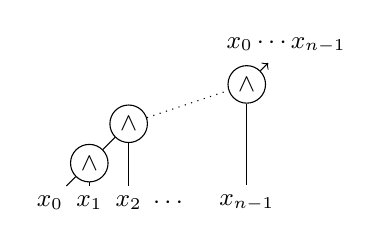
\begin{tikzpicture}[
    gate/.style={circle, draw, inner sep=2pt},
    every node/.style={font=\small}
]

% Inputs
\node (x0) at (-0.5,0) {$x_0$};
\node (x1) at (0,0) {$x_1$};
\node (x2) at (0.5,0) {$x_2$};
\node at (1,0) {$\cdots$};
\node (xn) at (2,0) {$x_{n-1}$};

% AND nodes
\node[gate] (a1) at (0,0.5) {$\wedge$};
\node[gate] (a2) at (0.5,1) {$\wedge$};
\node[gate] (ak) at (2,1.5) {$\wedge$};

% Output
\node (out) at (2.5,2) {$x_0\cdots x_{n-1}$};

% Edges
\draw (x0) -- (a1);
\draw (x1) -- (a1);
\draw (x2) -- (a2);

\draw (a1) -- (a2);
\draw[dotted] (a2) -- (ak);

\draw (xn) -- (ak);

\draw[->] (ak) -- (out);

\end{tikzpicture}



  }
  \caption{XAG for an MCT gate}
  \label{fig-mct-xag}
\end{figure}

This allows us to create a a quantum circuit based off the gadgets in~\tabref{fig-gadgets}. This is depicted
in~\figref{fig-mct-gadgets}. 

\begin{figure}[t]
  \centering
  \scalebox{1.0} {
    \begin{quantikz}[row sep=0.2em, column sep=0.5em]
\lstick{$x_1$}                & \ctrl{1}                   & \ctrl{1}                           & \qw               \\
\lstick{$x_2$}                & \ctrl{2}                   & \ctrl{2}                           & \qw               \\
\setwiretype{n}               & \setwiretype{n}            & \setwiretype{n}                    & \setwiretype{n}   \\
\lstick{$x_3$}                & \gate[2]{\wedge}           & \gate[2]{\wedge^{\dagger}}         & \qw                 \\
\lstick{$a_1$}                & \ghost{\wedge}\ctrl{1}     & \ghost{\wedge^{\dagger}}\ctrl{1}   & \qw               \\
\setwiretype{n}               &                            &                                    & \setwiretype{n}   \\
\setwiretype{n}\push{\vdots}  & \push{\vdots}              & \push{\vdots}                      & \setwiretype{n}   \\
\setwiretype{n}               &                            &                                    & \setwiretype{n}   \\
\lstick{$x_n$}                & \gate[2]{\wedge}\ctrl{-1}] & \vqw{-1}\vqw{1}                    & \qw               \\
\lstick{$a_{n-2}$}            & \ghost{\wedge}\ctrl{1}     & \targ[style={double}]{}            & \qw               \\
\lstick{$f$}                  & \targ{}                    & \qw                                &
\end{quantikz}

%% \begin{quantikz}[row sep=0.3cm, column sep=0.55cm]
%% \qw              & \qw             & \qw        & \qw             & \qw              & \gate[2]{F_i}       & \qw                    & \qw       & \qw             & \qw      & \qw        & \qw              & \gate[2]{F_i}        & \qw                     & \qw        \\
%% \qw              & \qw             & \qw        & \qw             & \qw              & \ghost{F_i}         & \qw                    & \qw       & \qw             & \qw      & \qw        & \qw              & \ghost{F_i}          & \qw                     & \qw        \\
%% \qw              & \qw             & \qw        & \qw             & \ctrl{2}         & \qw                 & \ctrl{2}               & \qw       & \qw             & \qw      & \qw        & \ctrl{2}         & \qw                 & \ctrl{2}                & \qw         \\
%% \qw              & \qw             & \octrl{2}  & \qw             & \qw              & \qw                 & \qw                    & \qw       & \qw             & \qw      & \qw        & \qw              & \qw                 & \qw                     & \qw         \\
%% \lstick{$a_1$}   & \qw             & \qw        & \qw             & \gate{i\omega Z} & \targ{}             & \gate{i\omega Z^\dagger} & \qw       & \octrl{1}       & \qw      & \qw        & \gate{i\omega Z} & \targ{}             & \gate{i\omega Z^\dagger}  & \qw          \\
%% \lstick{$a_2$}   & \qw             & \gate{iZ}  & \gate{H}        & \ctrl{-1}        & \qw                 & \ctrl{-1}              & \gate{H}  & \gate{iZ^\dagger} & \qw      & \gate{H}   & \ctrl{-1}        & \qw                 & \ctrl{-1}               & \gate{H}     \\
%% \lstick{}        & \gate{H}        & \ctrl{-1}  & \qw             & \qw              & \qw                 & \qw                    & \qw       & \ctrl{-1}       & \gate{H} & \qw        & \qw              & \qw                 & \qw                     & \qw          \\
%%\end{quantikz}


  }
  \caption{Synthesis of~\figref{fig-mct-xag} using dirty ancilla gadgets}
  \label{fig-mct-gadgets}
\end{figure}

This construction is remarkably similar to the ``V-chain'' that is created when the clean ancilla 
decomposition is used, such as in~\figref{fig-clean-mct}. This demonstrates that the difference in
cost between a dirty ancilla decomposition and a clean ancilla decomposition is the cost of the
final $\wedge$ gadget, which uses one more T-gate than the Toffoli gate that the clean ancilla
decomposition uses.




